\documentclass[12pt]{article}

\usepackage{sbc-template}
\usepackage{graphicx}
\usepackage[utf8]{inputenc}
\usepackage[brazil]{babel}


% Tema: Previsão da variação do fechamento do preço do BTC com relação ao fechamento do dia anterior
     
\sloppy

\title{Classificador de variação de criptomoedas com base no fechamento do dia anterior}

\author{Manoella Rockembach\inst{1} e Rodrigo Ferraz Souza\inst{1}}
%Luciana P. Nedel\inst{1}, Rafael H. Bordini\inst{2}, Flávio Rech
%  Wagner\inst{1}, Jomi F. Hübner\inst{3} 
 


\address{
Departamento de Computação -- Universidade Federal de Santa Catarina (UFSC)\\
 Araranguá -- SC -- Brasil
%\nextinstitute
%  Department of Computer Science -- University of Durham\\
%  Durham, U.K.
%\nextinstitute
%  Departamento de Sistemas e Computação\\
%  Universidade Regional de Blumenal (FURB) -- Blumenau, SC -- Brazil
%  \email{\{nedel,flavio\}@inf.ufrgs.br, R.Bordini@durham.ac.uk,
%  jomi@inf.furb.br}
}

\begin{document} 

\maketitle

\begin{resumo} 
  Este artigo propõe a utilização de redes neurais, sob o framework do TensorFlow, para resolver o problema de previsão da variação do fechamento do preço do Bitcoin. Nossos resultados mostram que, a partir dos dados que nós utilizamos, é impossível obter um resultado superior a jogar uma moeda para tentar prever os preços deste mercado.
  
\end{resumo}



\section{Problema Abordado}

Descrição do problema (introdução) ..

\section{Dados Utilizados} 

\begin{enumerate}
    \item Descrever se foram utilizados dados públicos, ou coletados a partir de pesquisa, ou foram base de dados cedidas.
    \item Quais as informações contidas na base de dados e quais foram utilizadas.
    \item Transformações necessárias nos dados.
\end{enumerate}

\subsection{teste2}
\subsubsection{teste1}
\subsection{teste}

\section{Solução do Problema}

\begin{itemize}
    \item Tipo de rede neural utilizada (exemplo, Perceptron), justificando a escolha e/ou necessidade.
    \item Critério de parada para o treinamento da rede.
    \item Avaliação de desempenho da rede.
\end{itemize}

\section{Conclusões}\label{sec:conclusao}

\textbf{Esse é um exemplo de citação}: segundo os autores em \cite{Russell2002LivroIA}, Inteligência Artificial é um tópico muito relevante em Ciência da Computação.

\begin{figure}[ht]
\centering
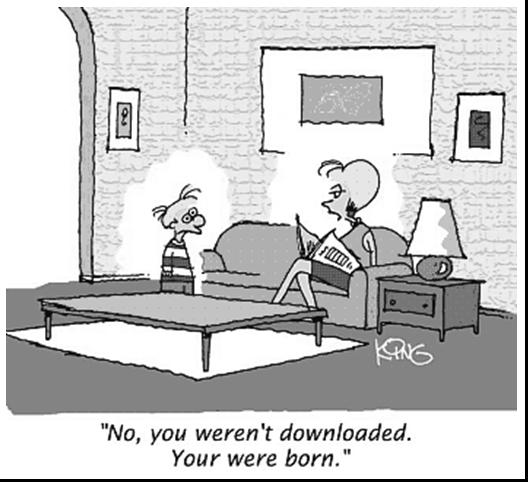
\includegraphics[width=.4\textwidth]{fig1.jpg}
\caption{Exemplo de Figura}
\label{fig:exampleFig1}
\end{figure}

Posso referenciar as figuras, tabelas e seções pelas suas labels, como a Figura~\ref{fig:exampleFig1}, na Seção~\ref{sec:conclusao}

Os autores em \cite{haykin2007redes} dizem que redes neurais são legais

\bibliographystyle{sbc}
\bibliography{sbc-template}

\end{document}
